% \begin{figure*}[t]
%   \centering
%   \begin{subfigure}[b]{0.48\linewidth}
%     \centering
%     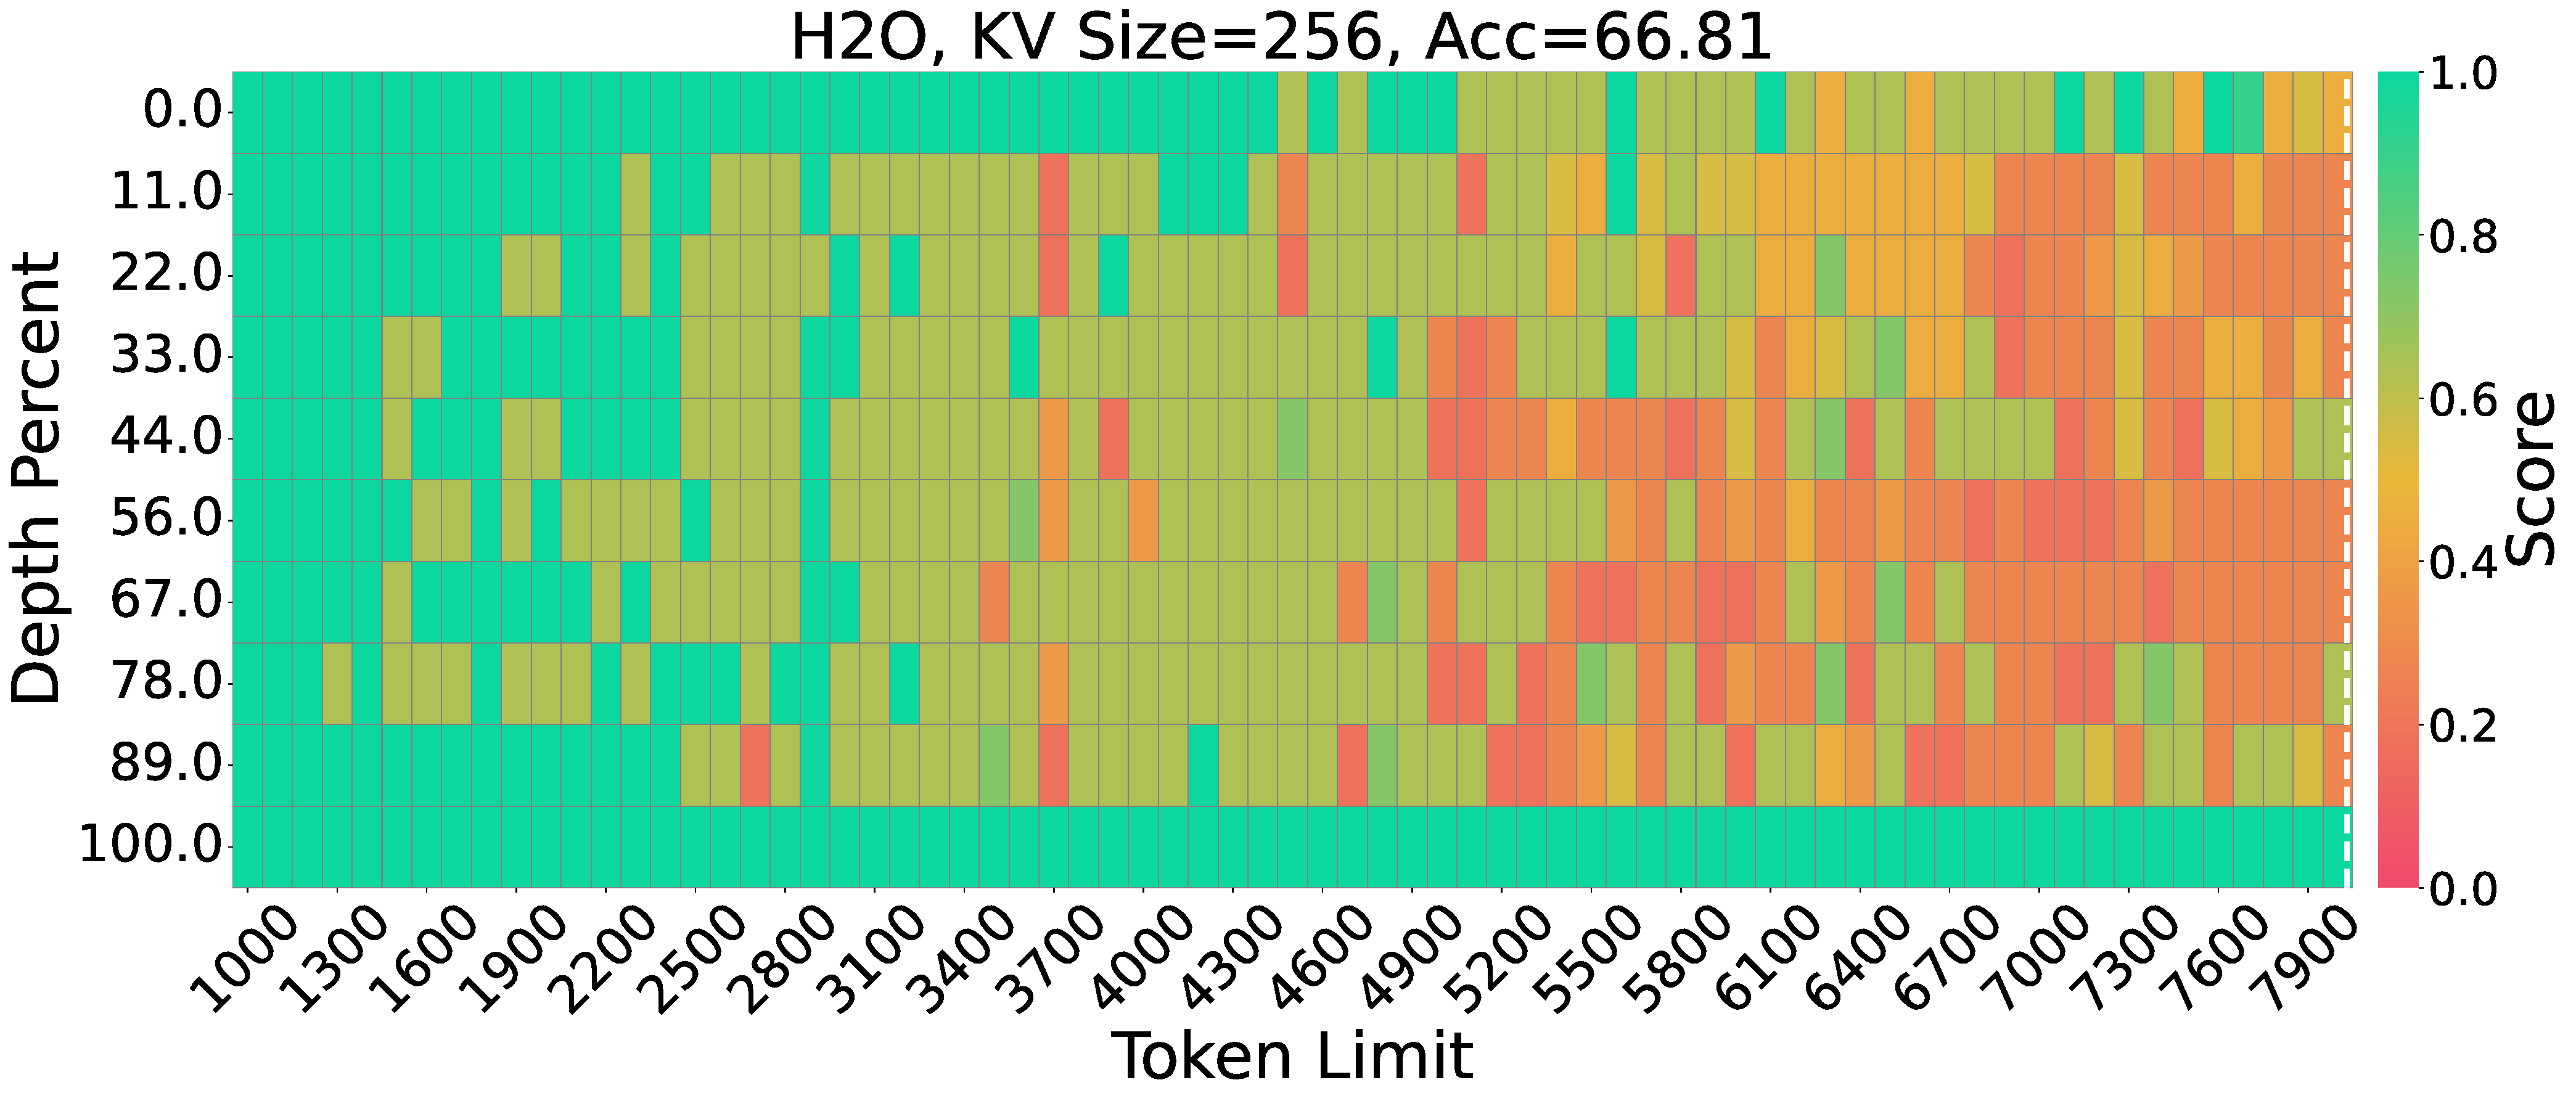
\includegraphics[width=\linewidth]{images/needle/llama-256/LlaMA3_h2o.pdf}
%     % \caption{H2O}
%   \end{subfigure}
%   \hfill
%   \begin{subfigure}[b]{0.48\linewidth}
%     \centering
%     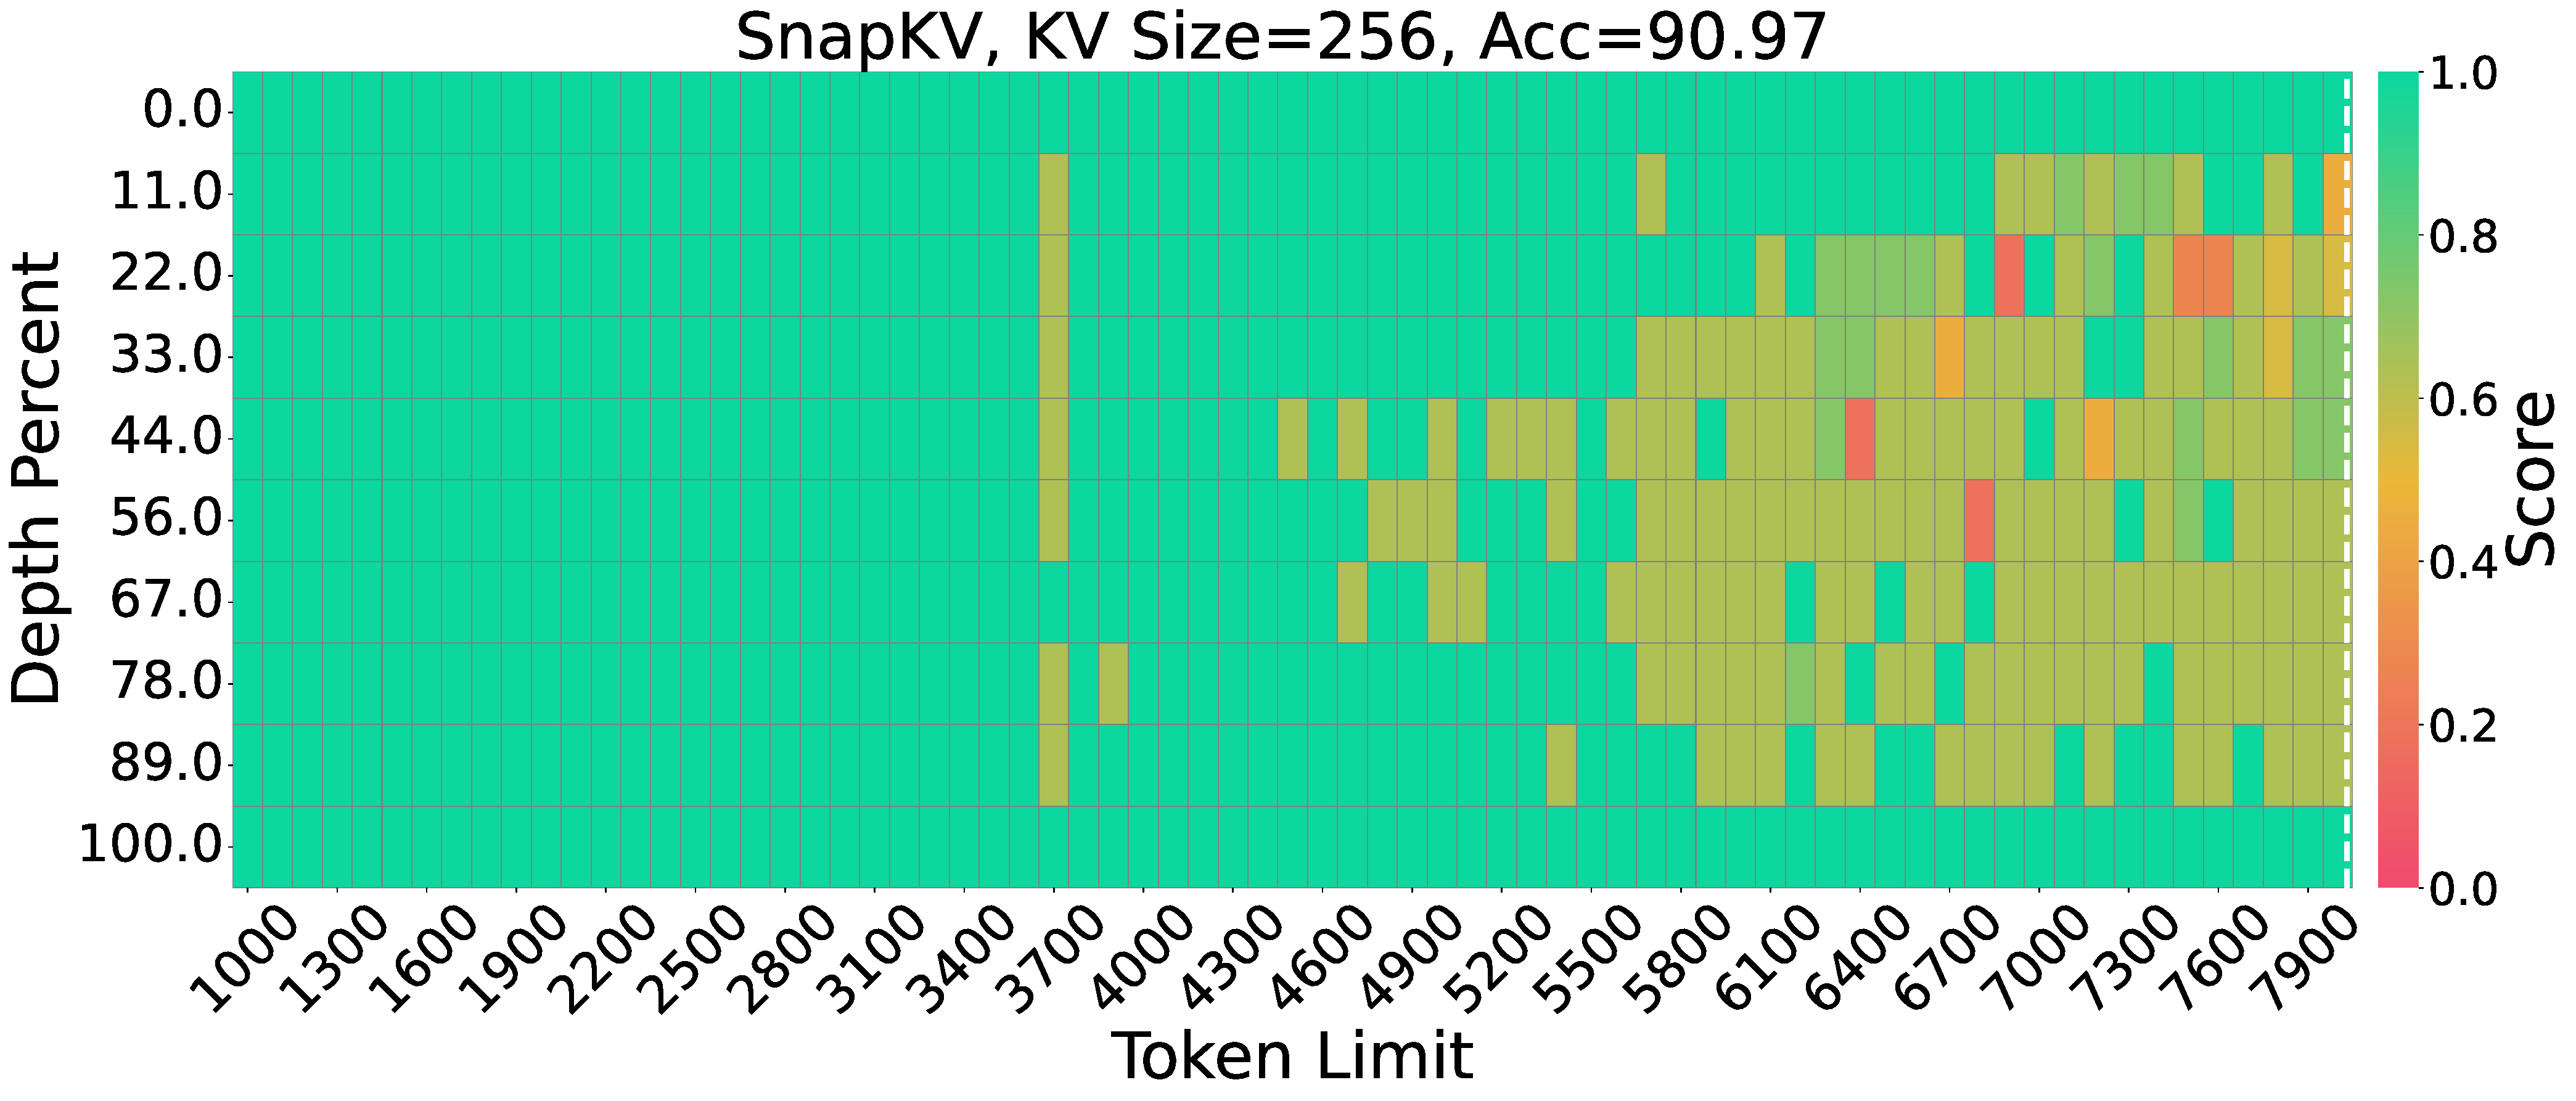
\includegraphics[width=\linewidth]{images/needle/llama-256/LlaMA3_snapkv.pdf}
%     % \caption{SnapKV}
%   \end{subfigure}
  
%   \vspace{0.1 cm}
  
%   \begin{subfigure}[b]{0.48\linewidth}
%     \centering
%     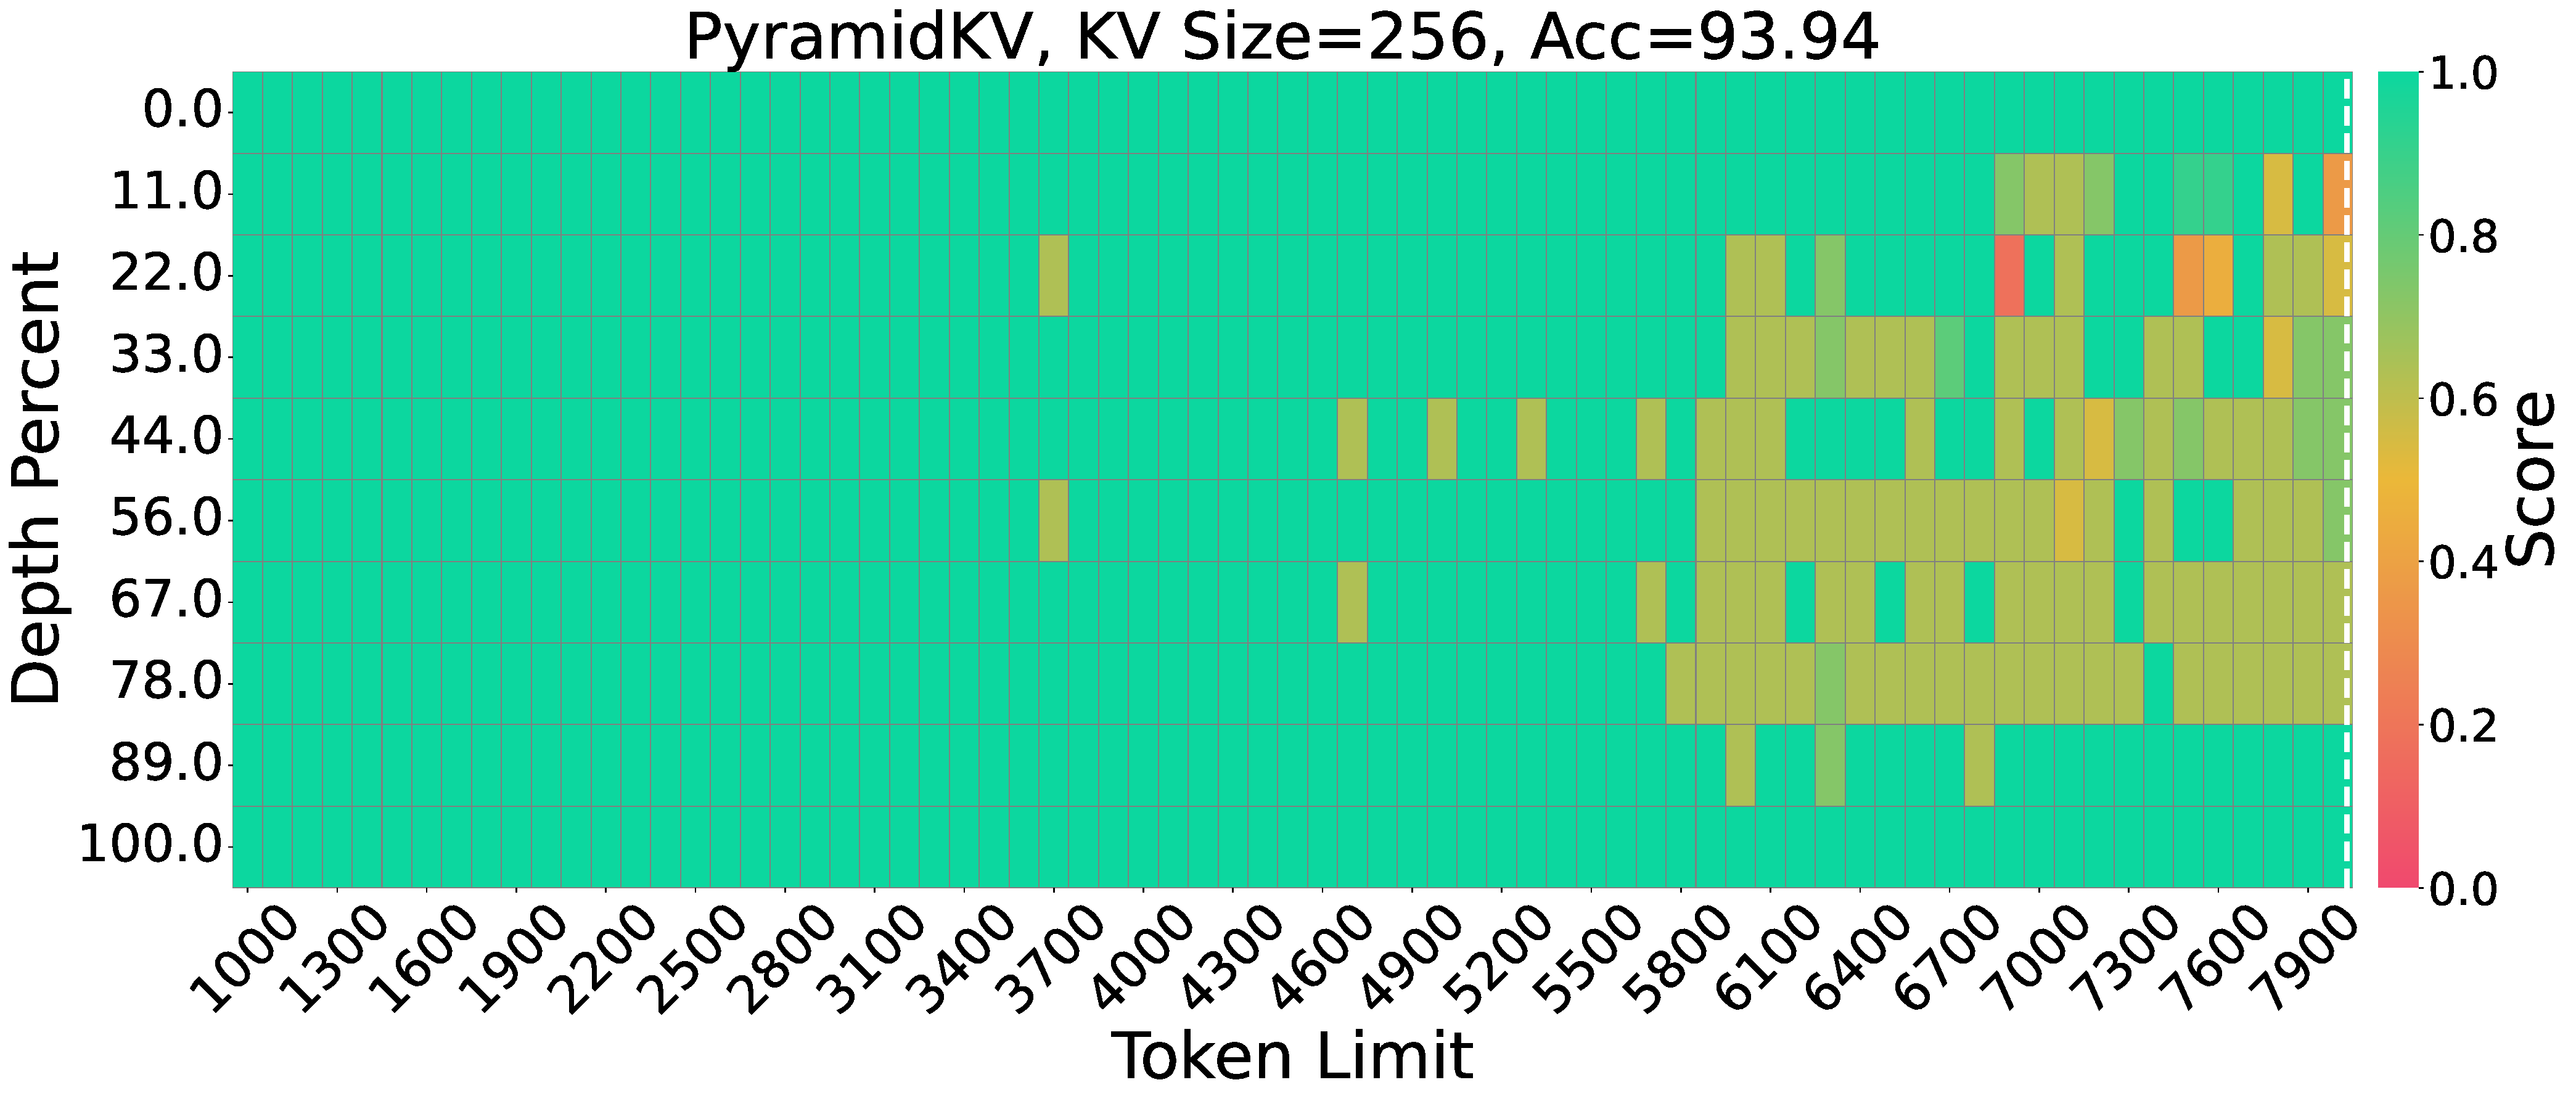
\includegraphics[width=\linewidth]{images/needle/llama-256/LlaMA3_pyramidkv.pdf}
%     % \caption{PyramidKV}
%   \end{subfigure}
%   \hfill
%   \begin{subfigure}[b]{0.48\linewidth}
%     \centering
%     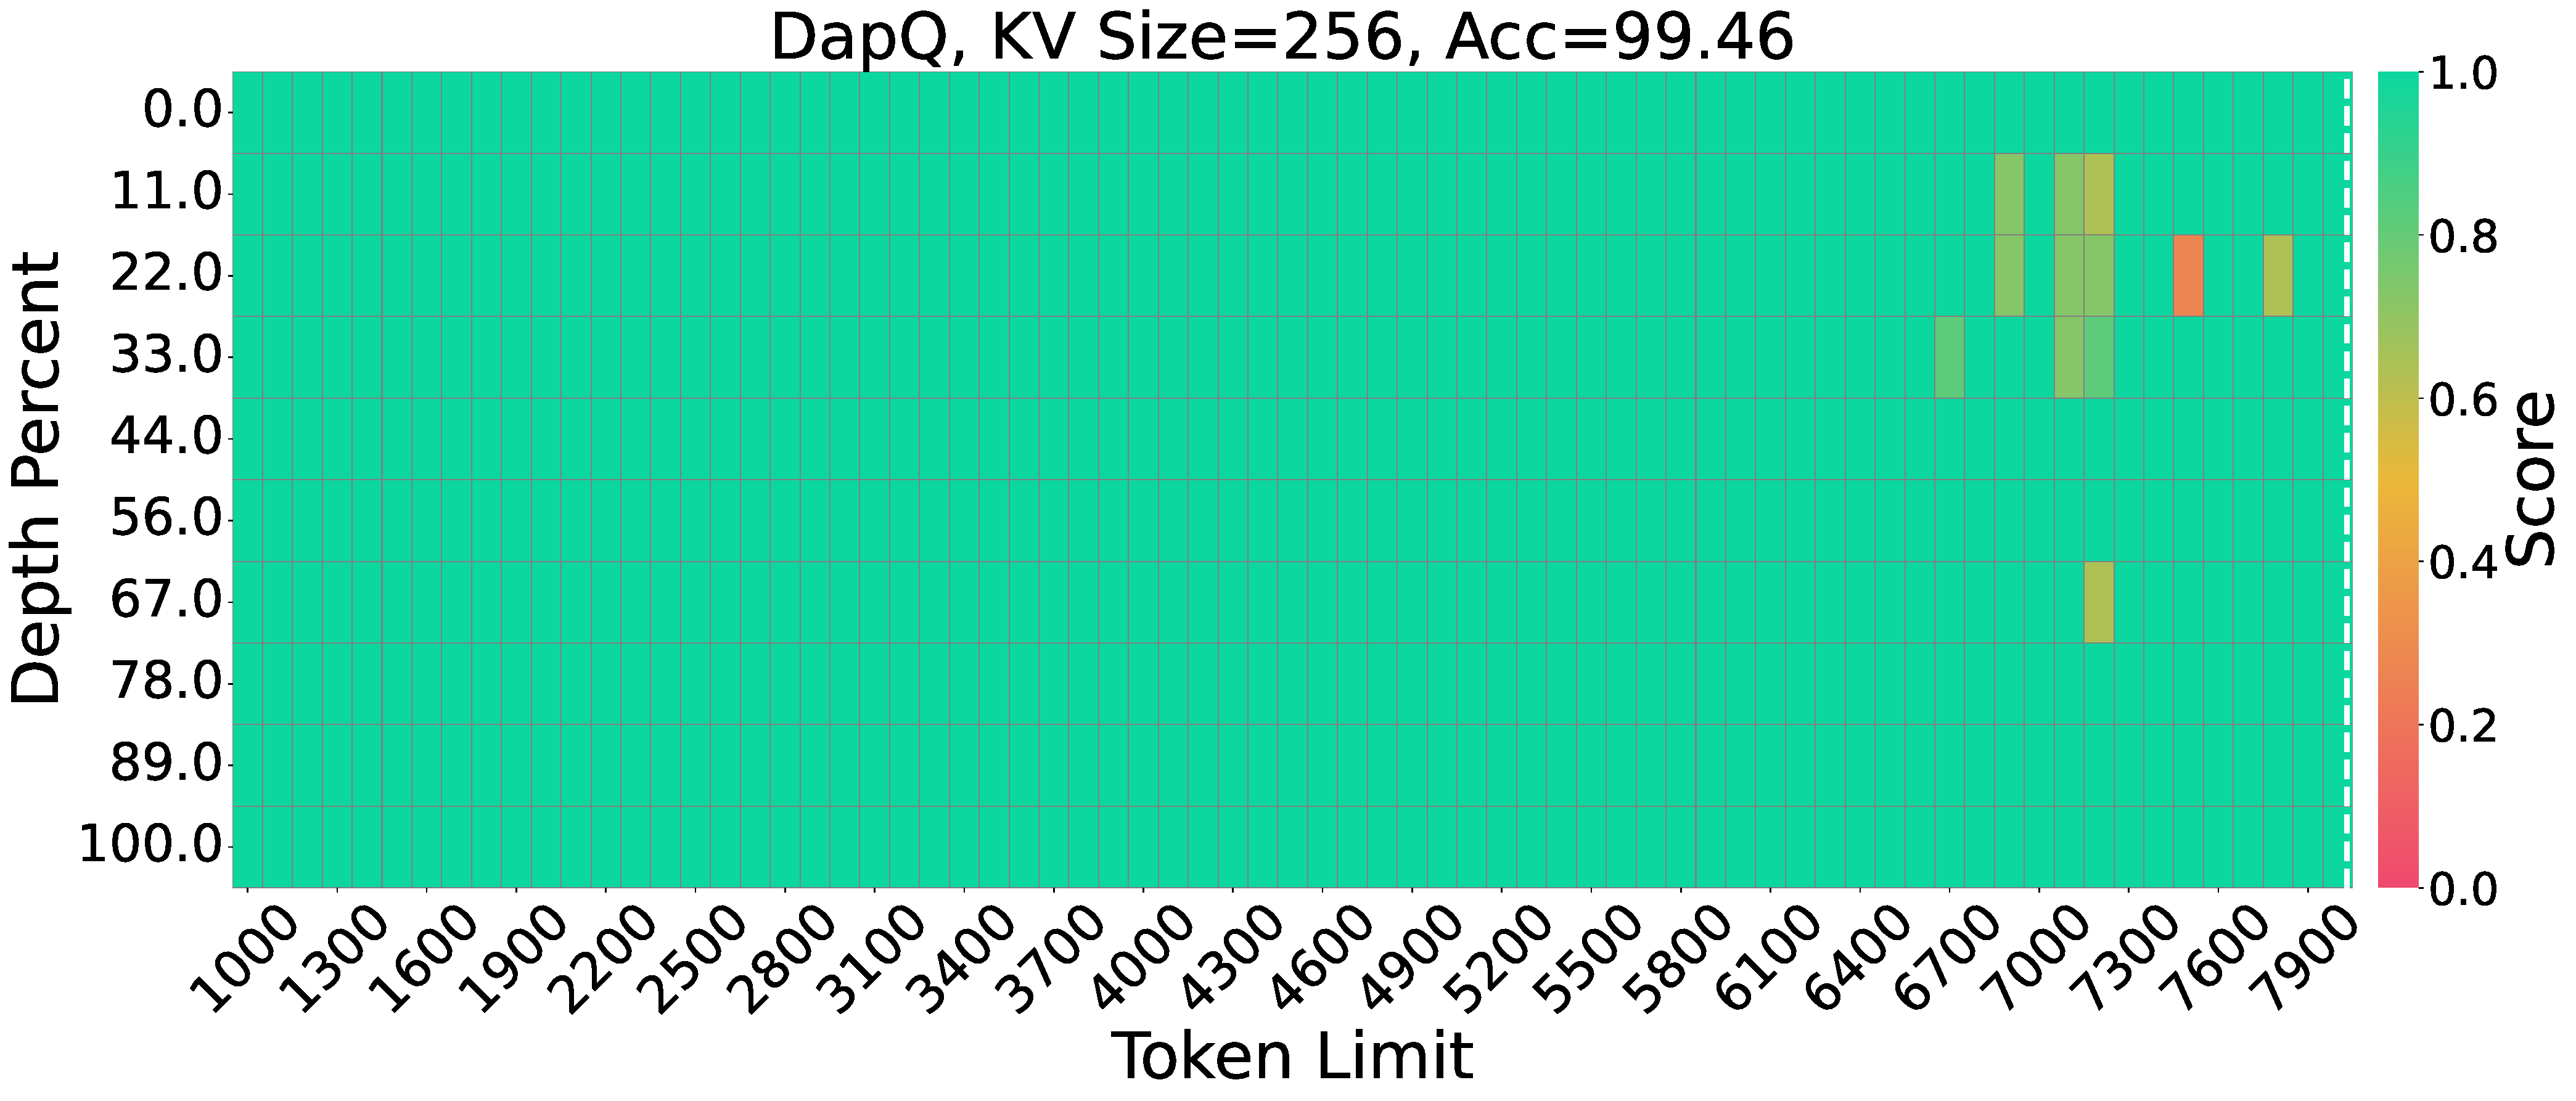
\includegraphics[width=\linewidth]{images/needle/llama-256/LlaMA3_ours.pdf}
%     % \caption{Ours}
%   \end{subfigure}
  
%   \caption{Results of Needle-in-a-Haystack on LLaMA-3-8B-Instruct with 8k context size and 256 KV size. The vertical axis of the figure represents the depth percentage, and the horizontal axis represents the token length.}
%   \vspace{-14pt}
%   \label{fig:needle}
% \end{figure*}


\begin{figure*}[t]
  \centering
  
  % 第一张图
  \begin{subfigure}[b]{0.7\linewidth} % 宽度设为0.7左右，居中显示
    \centering
    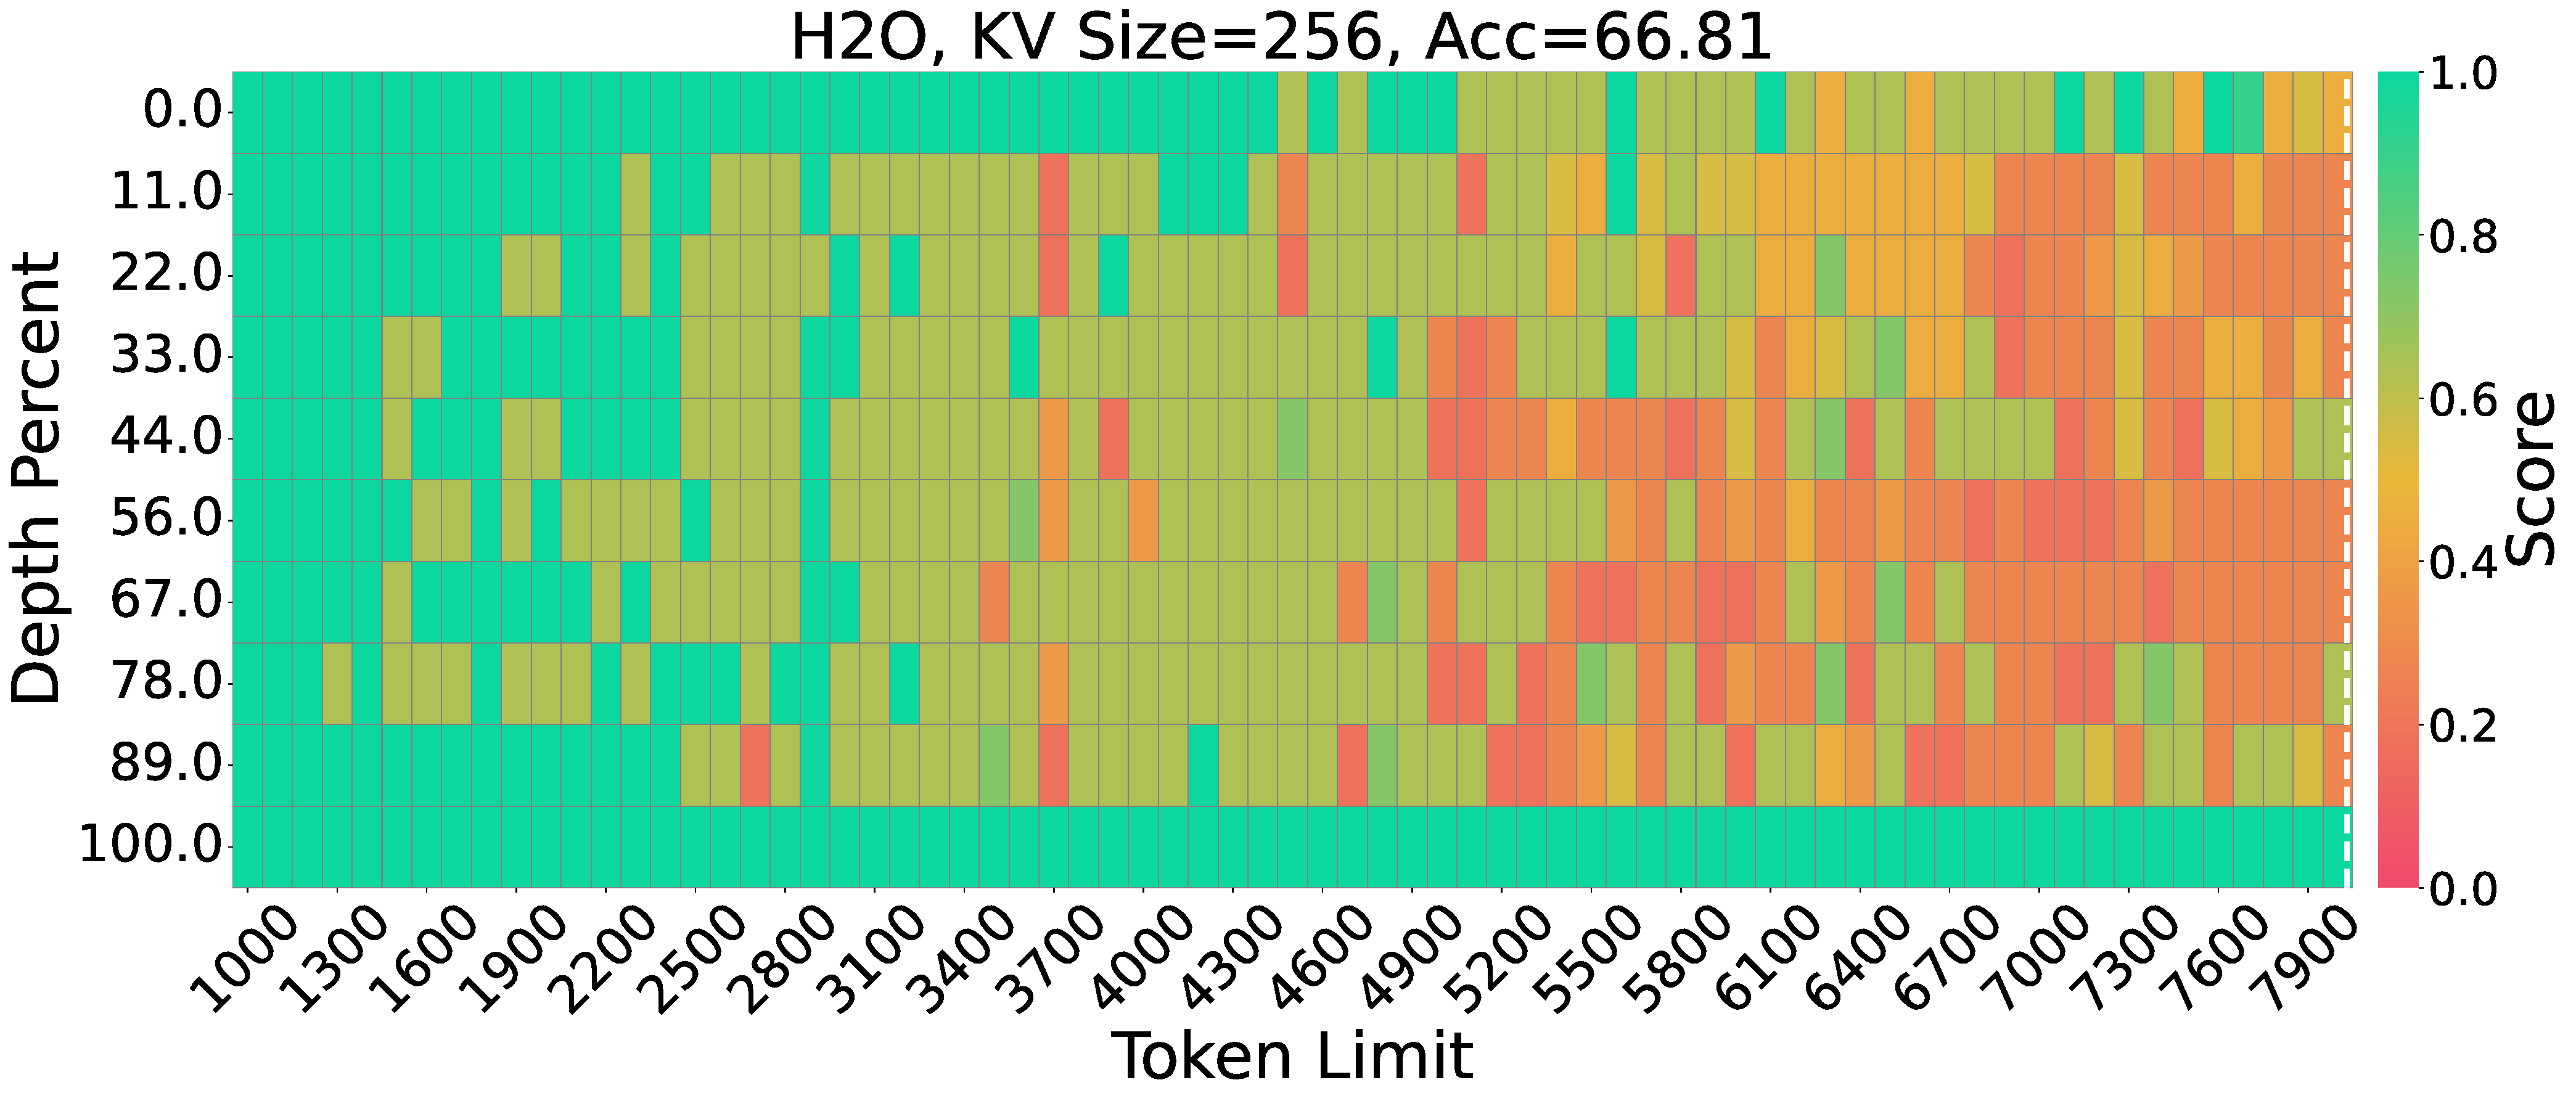
\includegraphics[width=\linewidth]{images/needle/llama-256/LlaMA3_h2o.pdf}
    % \caption{H2O}
  \end{subfigure}
  \par\vspace{0.2cm} % 【关键】强制换行 + 垂直间距
  
  % 第二张图
  \begin{subfigure}[b]{0.7\linewidth}
    \centering
    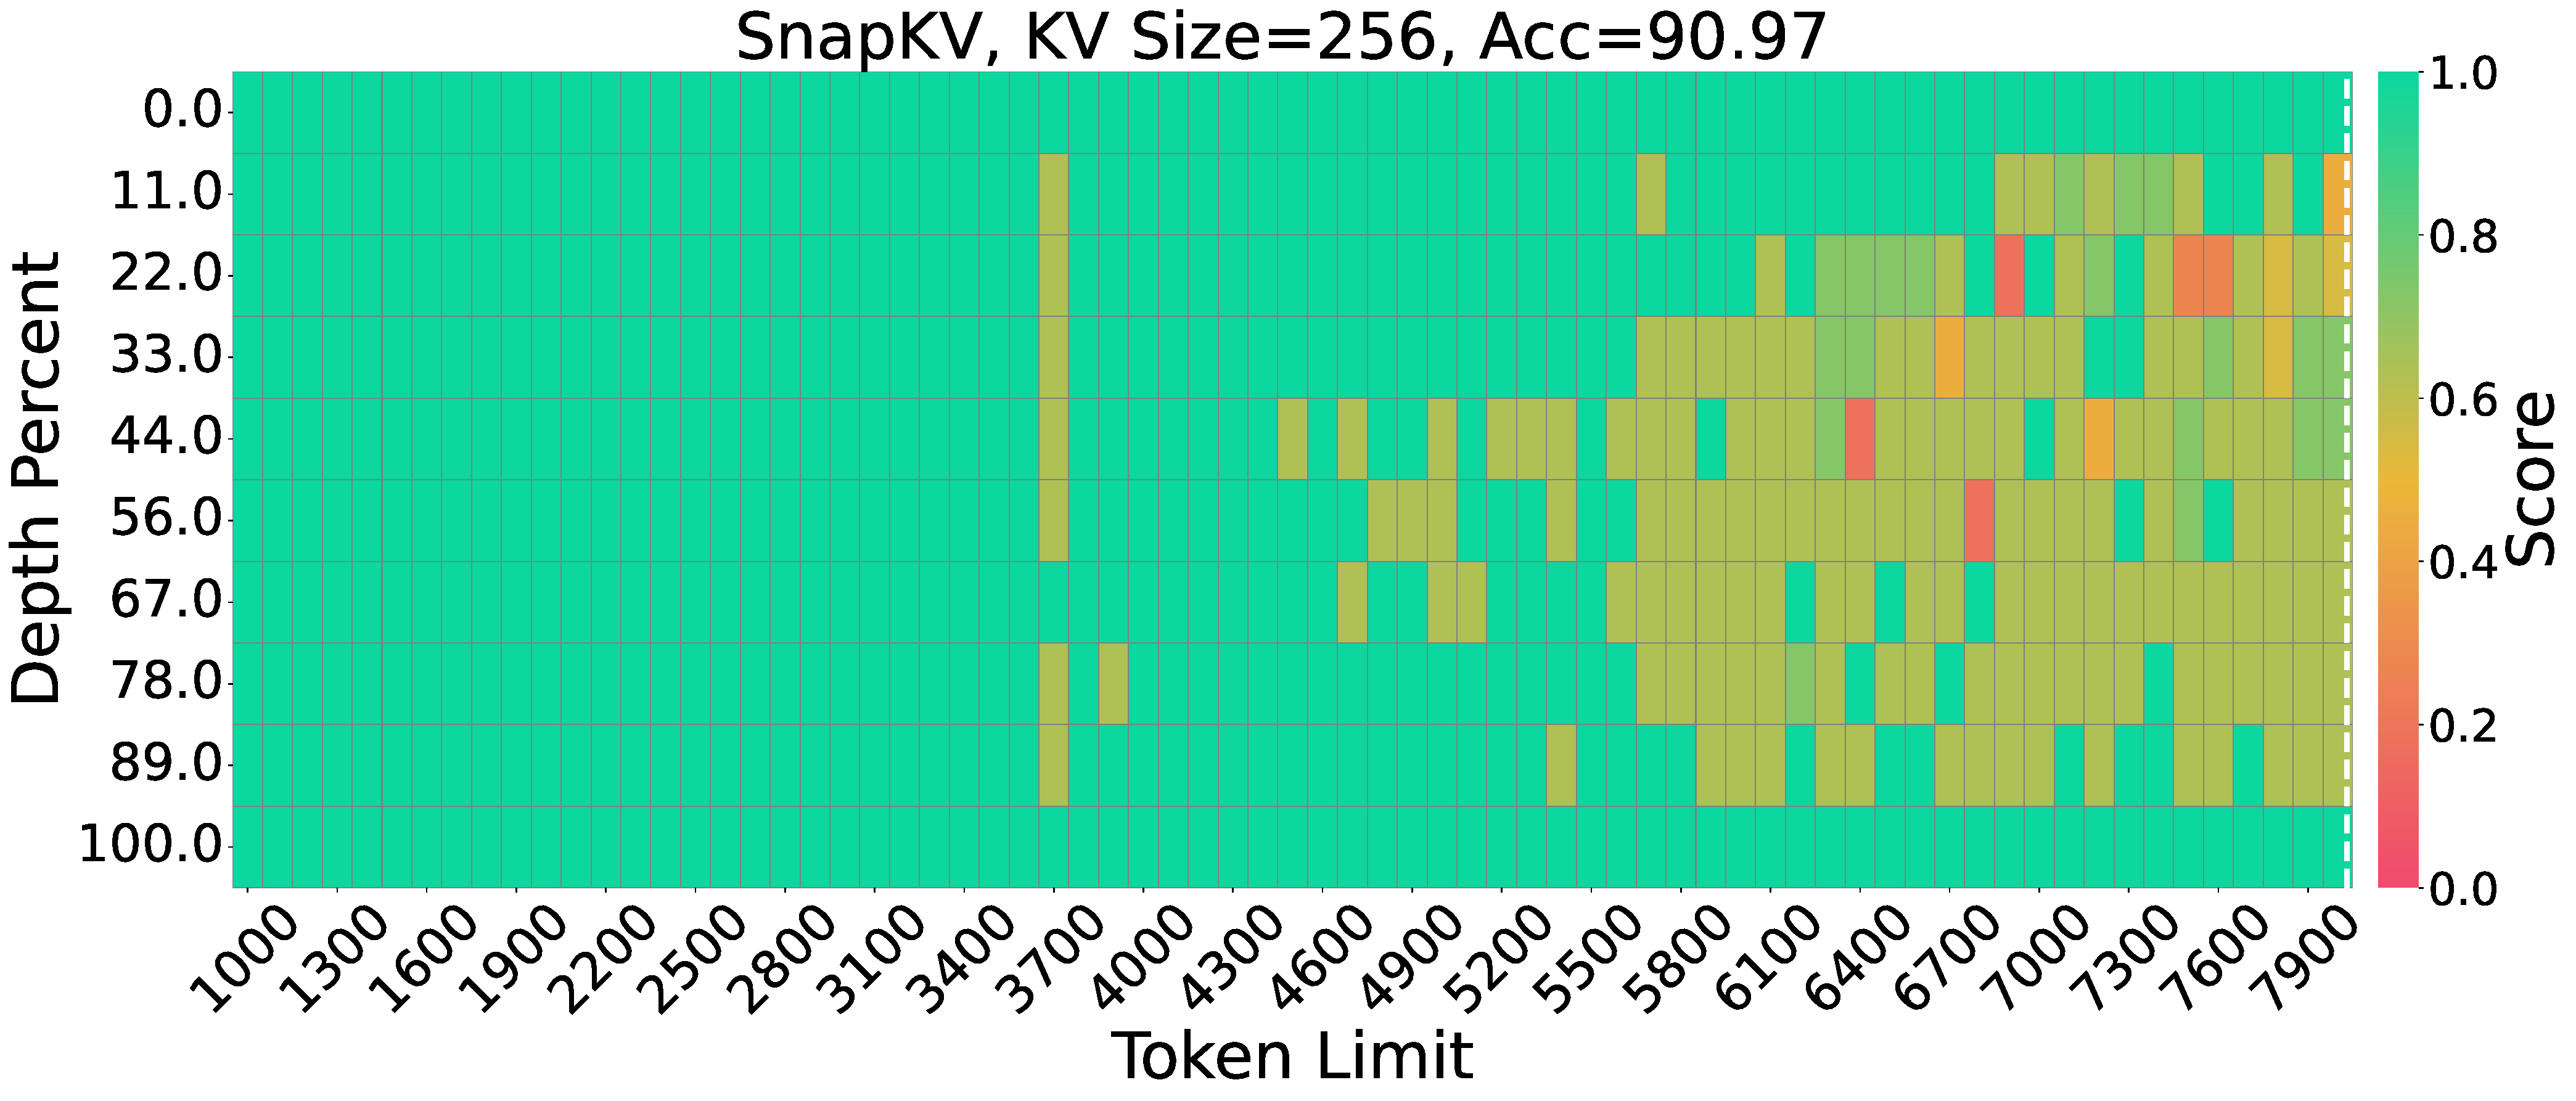
\includegraphics[width=\linewidth]{images/needle/llama-256/LlaMA3_snapkv.pdf}
    % \caption{SnapKV}
  \end{subfigure}
  \par\vspace{0.2cm}
  
  % 第三张图
  \begin{subfigure}[b]{0.7\linewidth}
    \centering
    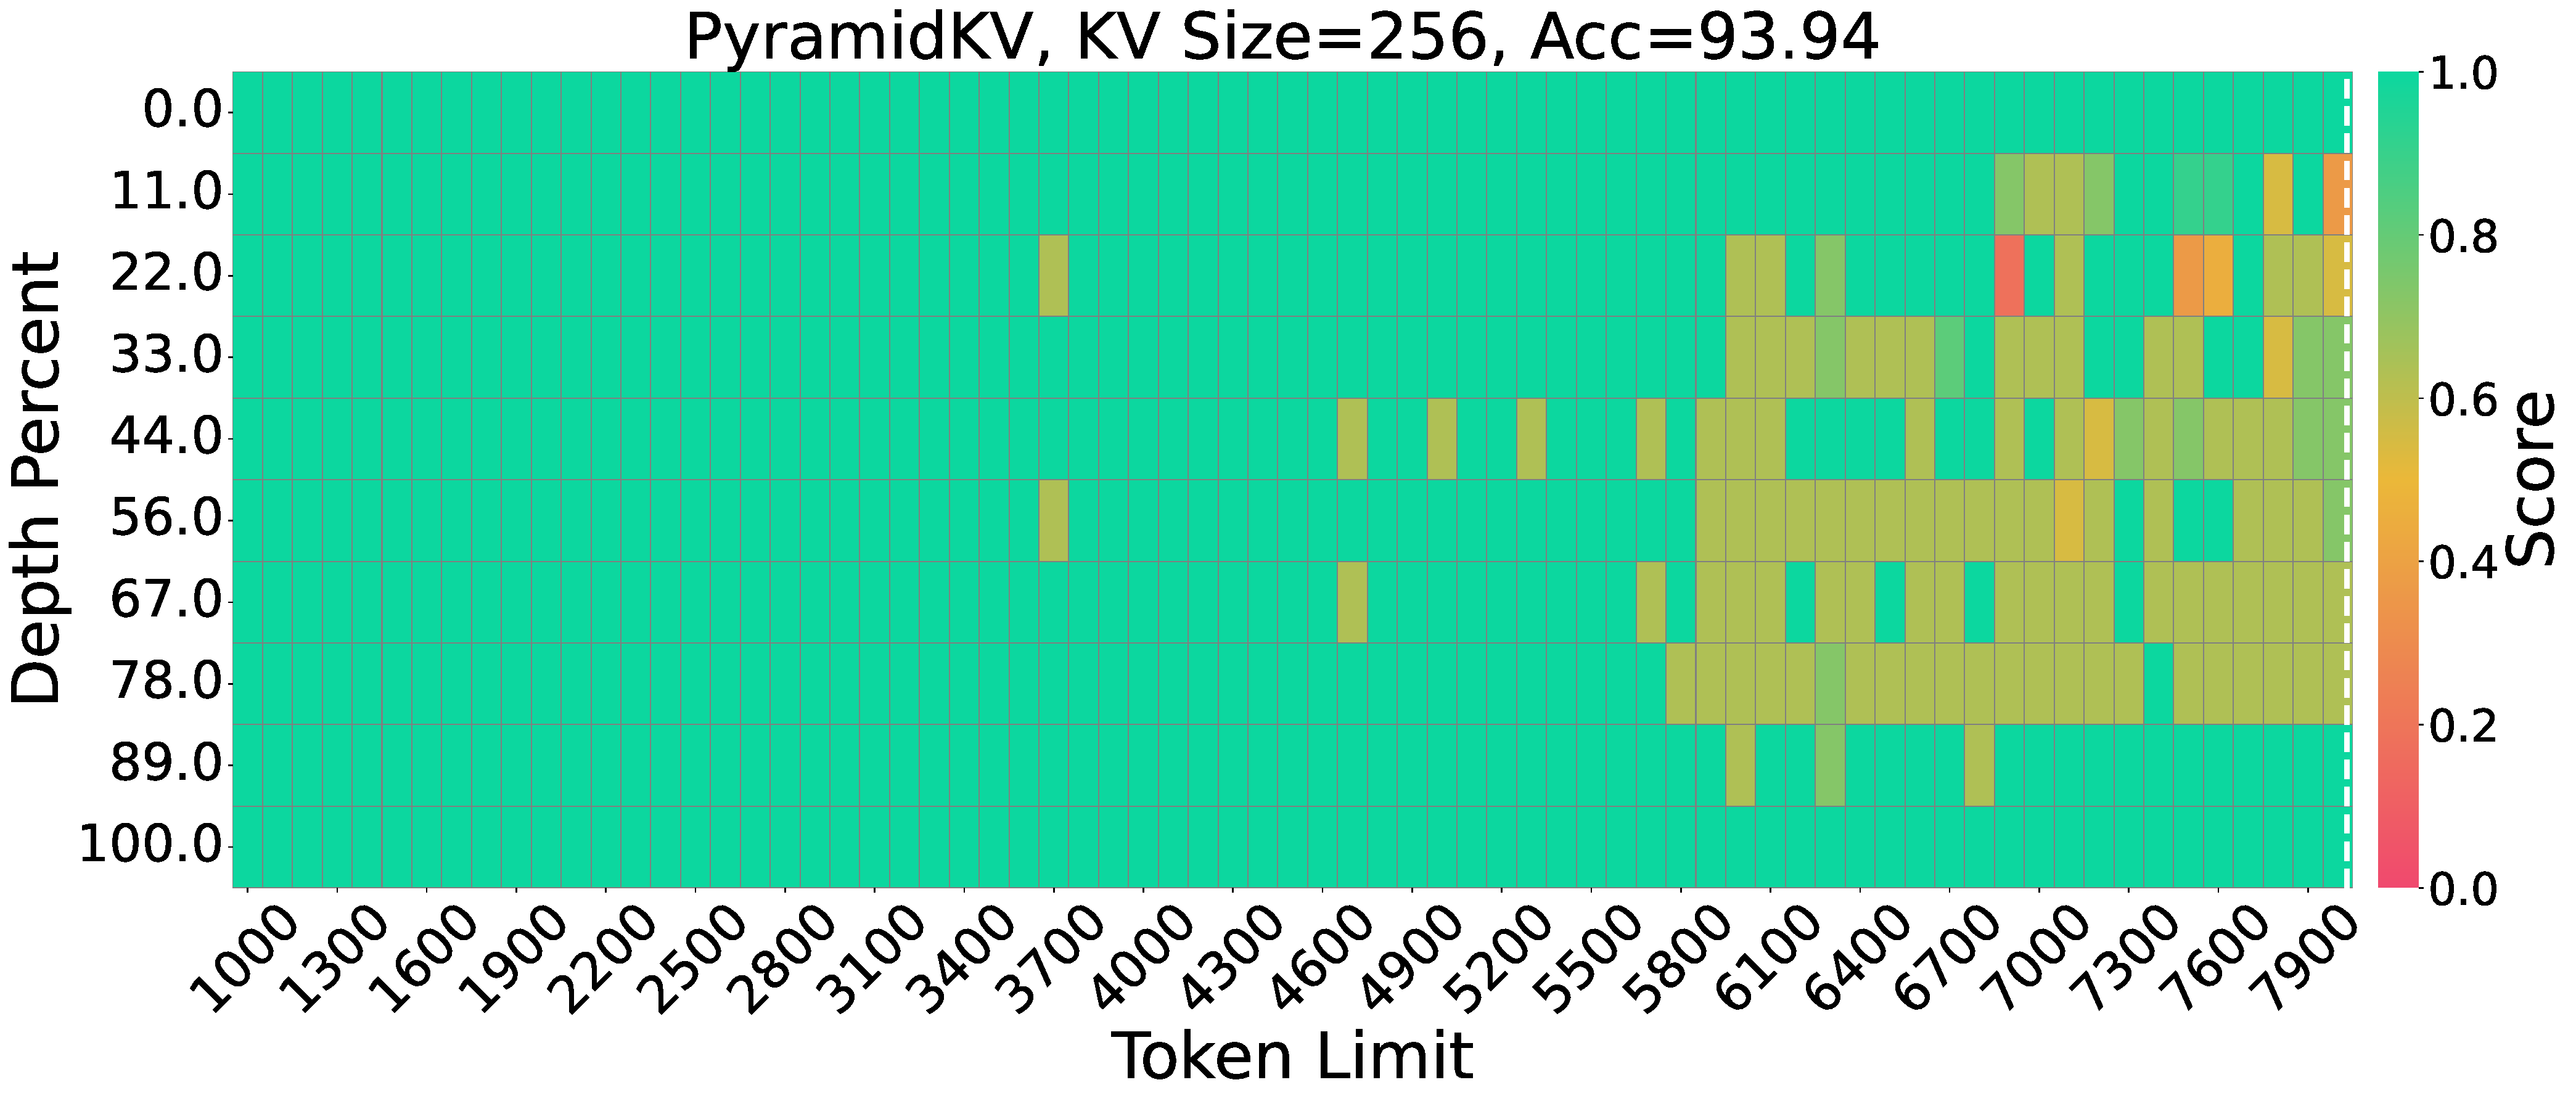
\includegraphics[width=\linewidth]{images/needle/llama-256/LlaMA3_pyramidkv.pdf}
    % \caption{PyramidKV}
  \end{subfigure}
  \par\vspace{0.2cm}
  
  % 第四张图
  \begin{subfigure}[b]{0.7\linewidth}
    \centering
    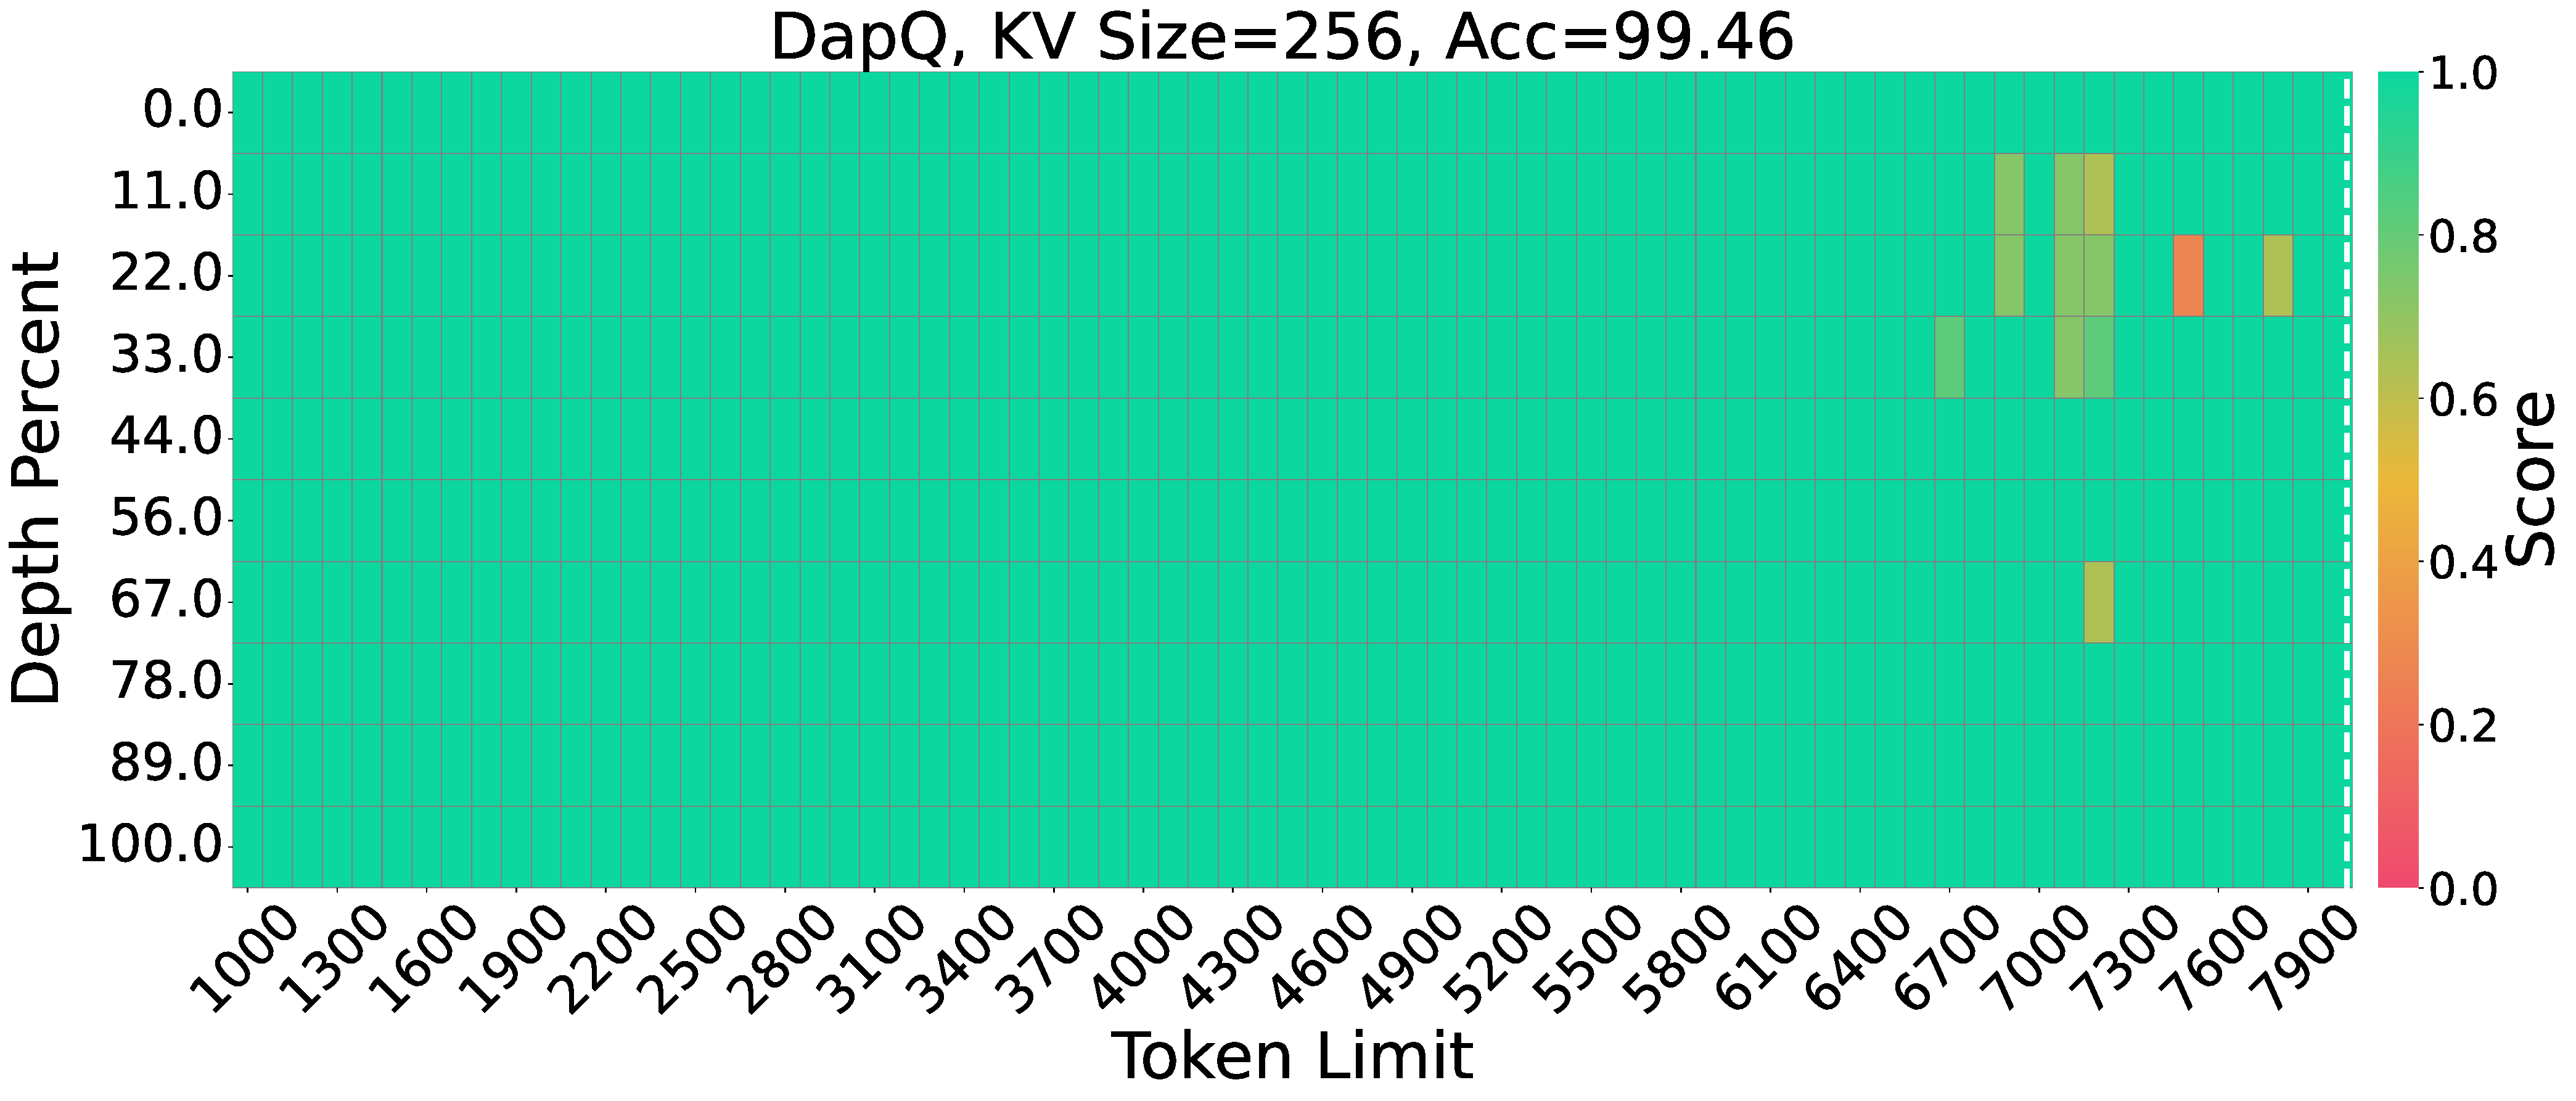
\includegraphics[width=\linewidth]{images/needle/llama-256/LlaMA3_ours.pdf}
    % \caption{Ours}
  \end{subfigure}
  
\caption{Visualization of Needle-in-a-Haystack results. We take LLaMA-3-8B-Instruct (8k context, 256 KV size) as a representative example to demonstrate the performance differences. The vertical axis represents the depth percentage, and the horizontal axis represents the token length.}
  \vspace{-14pt}
  \label{fig:needle}
\end{figure*}
